\ifx\flag\undefined
	\documentclass{easyclass}
	\begin{document}
\else
	\chapter{Quantum Gates}
\fi

This section studies quantum gates. As the basis, we begin with bit and qubit. We then discuss classical gates, reversible gates and quantum gates in turn. Last, we introduce the Bell circuit and its two applications, \textit{i.e.}, superdense coding and quantum teleportation.

\section{Bits and Qubits}
\label{sec:bits-and-qubits}
\begin{definition}[Bit]
	A \textbf{bit} is a unit of information describing a two-dimensional classical
	system.
\end{definition}

Since a two-dimensional classical system has two orthogonal states, hence the bit $0$ and bit $1$ can be represented as two $2\times 1$ binary vectors, \textit{i.e.},
\begin{equation}
	\textrm{bit-0}=\begin{bmatrix}1\\0 \end{bmatrix} \quad \textrm{and}\quad
	\textrm{bit-1}=\begin{bmatrix}0\\1 \end{bmatrix}
\end{equation}
where bit-0 and bit-1 equal to $\ket{0}$ and $\ket{1}$ for the convenience of the following discussion. 

\begin{definition}[Qubit]
	A \textbf{quantum bit} or a \textbf{qubit} is a unit of information describing a two- dimensional quantum system.
\end{definition}

\begin{figure}[h]
	\centering
	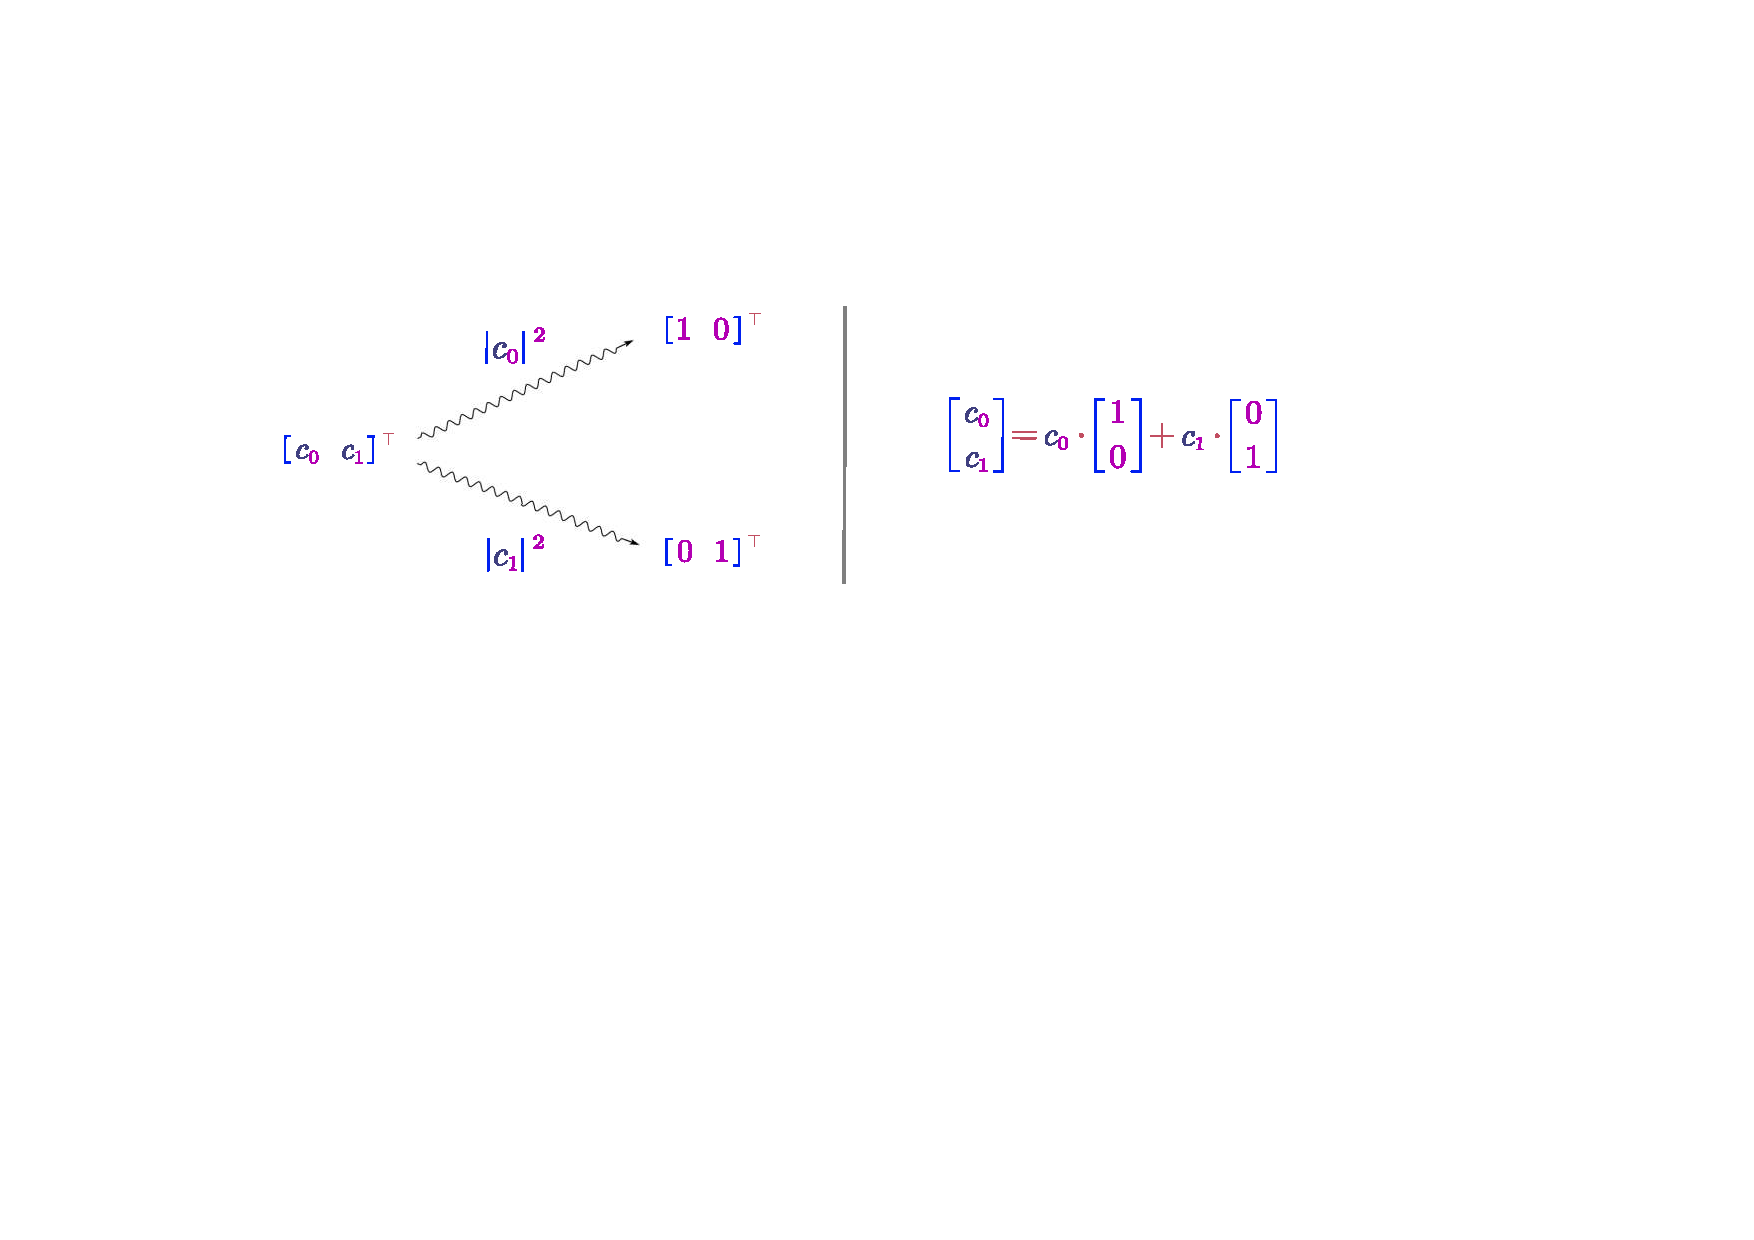
\includegraphics[width=0.75\textwidth]{qubit-bit}
	\caption{Relation between qubit and bit.}
	\label{fig:qubit-bit}
\end{figure}

The only difference between the above two definitions is the property of the two-dimensional system. The former is a classic system, while the latter is a quantum system. This means that the state of a qubit lies in the complex vector space satisfying the normalization constraint, \textit{i.e.},
\begin{equation}
	\ket{\varphi}=\begin{bmatrix}c_0\\c_1 \end{bmatrix}
\end{equation}
where $|c_0|^2+|c_1|^2=1$. Whenever we measure a qubit, it automatically becomes a bit with corresponding collapse probability of $|c_0|^2$ for bit $0$ and $|c_0|^2$ for bit $1$ as shown in Figure \ref{fig:qubit-bit}. So we shall never ``see'' a general qubit. 

\begin{definition}[Byte]
	The \textit{byte} is a unit of digital information that most commonly consists of eight bits.
\end{definition}

For example, given a byte including eight bits $01101011$, the vector representation of these eight bits is: $[1\ 0]^{\top}$, $[0\ 1]^{\top}$, $[0\ 1]^{\top}$, $[1\ 0]^{\top}$,  $[0\ 1]^{\top}$,  $[1\ 0]^{\top}$, $[0\ 1]^{\top}$,  $[0\ 1]^{\top}$. Recall the tensor product in composite system, the state of a byte equals to $\ket{0}\otimes \ket{1}\otimes \ket{1}\otimes \ket{0}\otimes \ket{1}\otimes \ket{0}\otimes \ket{1}\otimes \ket{1}$, which is a discrete element of the complex vector space $\mathbb{C}^2\otimes\mathbb{C}^2\otimes\mathbb{C}^2\otimes\mathbb{C}^2\otimes\mathbb{C}^2\otimes\mathbb{C}^2\otimes\mathbb{C}^2\otimes\mathbb{C}^2$.

\begin{definition}[Qubyte]
	The \textit{qubyte} is a unit of quantum information that consists of eight qubits.
\end{definition}

Similar, the state of a qubyte is the tensor product of eight qubits, \textit{i.e.}, $\ket{\varphi_0}\otimes\ket{\varphi_1}\otimes\ket{\varphi_2}\otimes\ket{\varphi_3}\otimes\ket{\varphi_4}\otimes\ket{\varphi_5}\otimes\ket{\varphi_6}\otimes\ket{\varphi_7}$, wihch is a continues element of the complex vector space $\mathbb{C}^2\otimes\mathbb{C}^2\otimes\mathbb{C}^2\otimes\mathbb{C}^2\otimes\mathbb{C}^2\otimes\mathbb{C}^2\otimes\mathbb{C}^2\otimes\mathbb{C}^2$.

\begin{figure}[h]
	\centering
	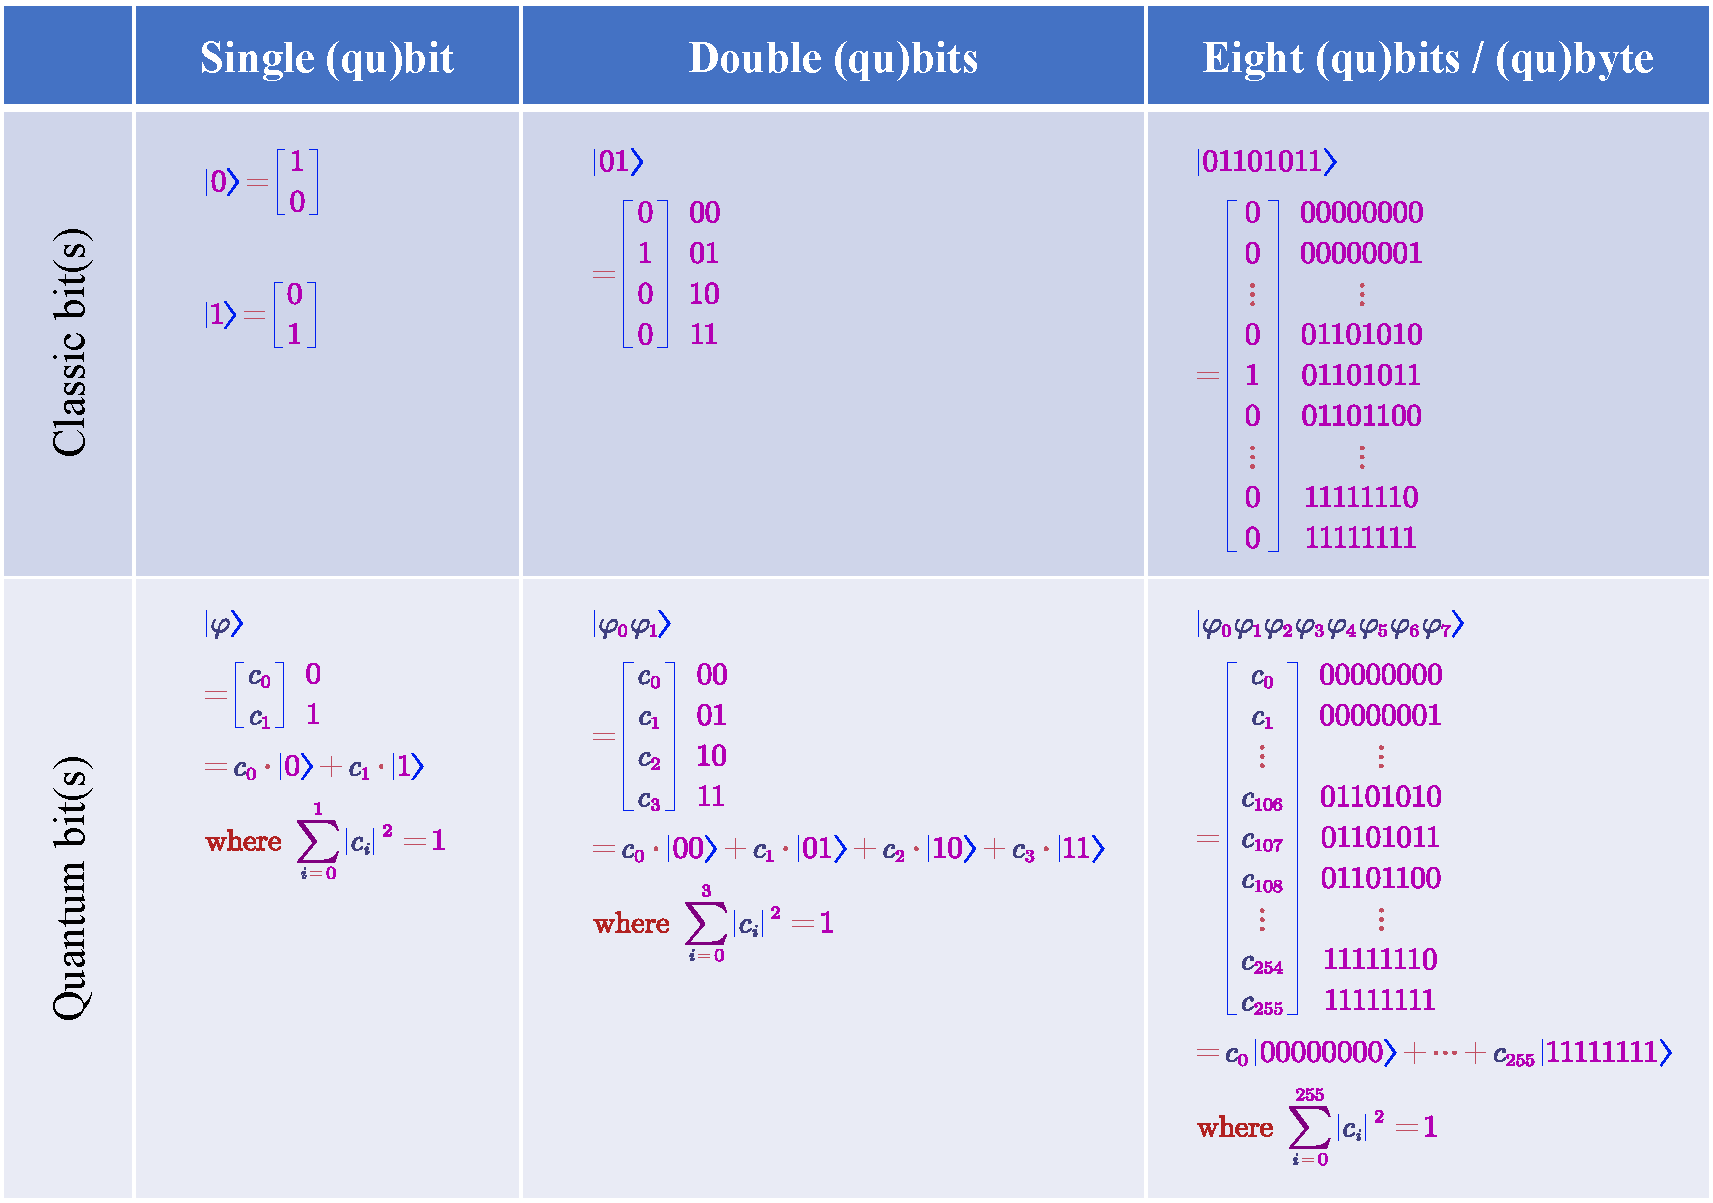
\includegraphics[width=\textwidth]{bits-state}
	\caption{State vectors of single (qu)bit, double (qu)bits and (qu)byte.}
	\label{fig:bits-state}
\end{figure}

The state vectors of single (qu)bit, double (qu)bits and (qu)byte are shown in Figure \ref{fig:bits-state}. Let's compare the byte and qubyte, both of them are represented as a $256$-dimensional vector. But the former, classic byte, contains only $8$ binary numbers, while the latter, quantum byte, contains $2^8=256$ complex numbers. This difference indicates qubyte is much more informative than the classic byte.

\section{Classic Gates}
\textbf{Matrix representation.} Classical logical gates are ways of manipulating bits. This section studies classical gates from the point of view of matrices. As stated in Section \ref{sec:bits-and-qubits}, we represent $n$ input bits as a $2^n\times 1$ vector and $m$ output bits as a $2^m\times 1$ vector. How should we represent our logical gates? When one multiplies a $2^m\times 2^n$ matrix with a $2^n\times 1$ vector, the result is a $2^m\times 1$ vector. In symbols:
\begin{equation}
	\underbrace{(2^m\times 2^n)}_{\textrm{\color{red} gate}}\cdot\underbrace{(2^n\times 1)}_{\textrm{input}} = \underbrace{(2^m\times 1)}_{\textrm{output}}
\end{equation}

\begin{example}[NOT gate]{ex:NOT-gate}
	Consider the NOT gate:
	\begin{minipage}{\textwidth}
		\begin{circuitikz}
			\draw (0,0) node[not port] (mynot) {};
			\draw (mynot.in) node[left] {$A$};
			\draw (mynot.out) node[right] {$Y$};
		\end{circuitikz}
	\end{minipage}	

	NOT gate takes as input one bit, or a $2\times 1$ vector, and outputs one bit, or a $2\times 1$ vector. NOT of $\ket{0}$ equals $\ket{1}$ and NOT of $\ket{1}$ equals $\ket{0}$. Consider the matrix
	\begin{equation}
		\mathrm{NOT}=\begin{bmatrix}
			0 & 1\\
			1 & 0
		\end{bmatrix}
	\end{equation}
	This matrix satisfies
	\begin{equation}
		\begin{bmatrix}
			0 & 1\\
			1 & 0
		\end{bmatrix}
		\begin{bmatrix}
			1\\
			0
		\end{bmatrix}=
		\begin{bmatrix}
			0\\
			1
		\end{bmatrix}
		\quad \textrm{and} \quad
		\begin{bmatrix}
			0 & 1\\
			1 & 0
		\end{bmatrix}
		\begin{bmatrix}
			0\\
			1
		\end{bmatrix}=
		\begin{bmatrix}
			1\\
			0
		\end{bmatrix}
	\end{equation} 
\end{example}


\begin{example}[AND gate]{ex:AND-gate}
	Consider the AND gate:
	\begin{minipage}{\textwidth}
		\begin{circuitikz}
			\draw (0,0) node[and port] (myand) {};
			\draw (myand.in 1) node[left] {$A$};
			\draw (myand.in 2) node[left] {$B$};
			\draw (myand.out) node[right] {$Y$};
		\end{circuitikz}
	\end{minipage}	
	
	The AND gate accepts two bits and outputs one bit, hence we need a $2^1\times 2^2$ matrix. Consider the matrix
	\begin{equation}
		\mathrm{AND}=\begin{bmatrix}
			1 & 1 & 1 & 0\\
			0 & 0 & 0 & 1
		\end{bmatrix}
	\end{equation}
	This matrix satisfies $\textrm{AND}\ket{11}=\ket{1}$ and $\textrm{AND}\ket{01}=\ket{0}$
	\begin{equation}
		\begin{bmatrix}
			1 & 1 & 1 & 0\\
			0 & 0 & 0 & 1
		\end{bmatrix}
		\begin{bmatrix}
			0\\ 0\\ 0\\ 1
		\end{bmatrix}=
		\begin{bmatrix}
			0\\ 1
		\end{bmatrix}
		\quad \textrm{and} \quad
		\begin{bmatrix}
			1 & 1 & 1 & 0\\
			0 & 0 & 0 & 1
		\end{bmatrix}
		\begin{bmatrix}
			0\\ 1\\ 0\\ 0
		\end{bmatrix}=
		\begin{bmatrix}
			1\\ 0
		\end{bmatrix}
	\end{equation} 	
\end{example}

\begin{example}[OR gate]{ex:OR-gate}
	Consider the OR gate:
	\begin{minipage}{\textwidth}
		\begin{circuitikz}
			\draw (0,0) node[or port] (myor) {};
			\draw (myor.in 1) node[left] {$A$};
			\draw (myor.in 2) node[left] {$B$};
			\draw (myor.out) node[right] {$Y$};
		\end{circuitikz}
	\end{minipage}	
	
	The OR gate similarly accepts two bits and outputs one bit, hence can be represented by a $2^1\times 2^2$ matrix. 
	\begin{equation}
		\mathrm{AND}=\begin{bmatrix}
			1 & 0 & 0 & 0\\
			0 & 1 & 1 & 1
		\end{bmatrix}
	\end{equation}
	This matrix satisfies $\textrm{OR}\ket{00}=\ket{0}$ and $\textrm{AND}\ket{01}=\ket{1}$
	\begin{equation}
		\begin{bmatrix}
			1 & 0 & 0 & 0\\
			0 & 1 & 1 & 1
		\end{bmatrix}
		\begin{bmatrix}
			1\\ 0\\ 0\\ 0
		\end{bmatrix}=
		\begin{bmatrix}
			1\\ 0
		\end{bmatrix}
		\quad \textrm{and} \quad
		\begin{bmatrix}
			1 & 0 & 0 & 0\\
			0 & 1 & 1 & 1
		\end{bmatrix}
		\begin{bmatrix}
			0\\ 1\\ 0\\ 0
		\end{bmatrix}=
		\begin{bmatrix}
			0\\ 1
		\end{bmatrix}
	\end{equation} 	
\end{example}


\begin{example}[NAND gate]{ex:NAND-gate}
	Consider the NAND gate:
	\begin{minipage}{\textwidth}
		\begin{circuitikz}
			\draw (0,0) node[nand port] (mynand) {};
			\draw (mynand.in 1) node[left] {$A$};
			\draw (mynand.in 2) node[left] {$B$};
			\draw (mynand.out) node[right] {$Y$};
		\end{circuitikz}
	\end{minipage}	
	
	The NAND gate similarly accepts two bits and outputs one bit, hence can be represented by a $2^1\times 2^2$ matrix. 
	\begin{equation}
		\mathrm{AND}=\begin{bmatrix}
			0 & 0 & 0 & 1\\
			1 & 1 & 1 & 0
		\end{bmatrix}
	\end{equation}
	This matrix satisfies $\textrm{NOT}\times\textrm{AND}=\textrm{NAND}$
	\begin{equation}
		\textrm{NOT}\cdot\textrm{AND}=
		\begin{bmatrix}
			0 & 1\\
			1 & 0
		\end{bmatrix}
		\begin{bmatrix}
			1 & 1 & 1 & 0\\
			0 & 0 & 0 & 1
		\end{bmatrix}=
		\begin{bmatrix}
			0 & 0 & 0 & 1\\
			1 & 1 & 1 & 0
		\end{bmatrix}=\textrm{NAND}
	\end{equation} 	
\end{example}

\textbf{Sequential operation.} The way of thinking of NAND brings to light a general situation. When we perform a computation, we often have to carry out one operation followed by another. We call this procedure performing \textbf{sequential} operations. Take Figure \ref{subfig:sequential} as an example, if A an operation with $m$ input bits and $n$ output bits, its matrix will be of size $2^n\times 2^m$. Say, B takes the $n$ outputs of A as input and outputs $p$ bits, then B is represented by a $2^p\times 2^n$ matrix, and performing one operation sequentially followed by another operation corresponds to $\textrm{B} \times \textrm{A}$, which is a $(2^p\times 2^n)\times(2^n\times 2^m) = (2^p\times 2^m)$ matrix.

\begin{figure}[h]
	\centering
	\subfloat[Sequential operation]
	{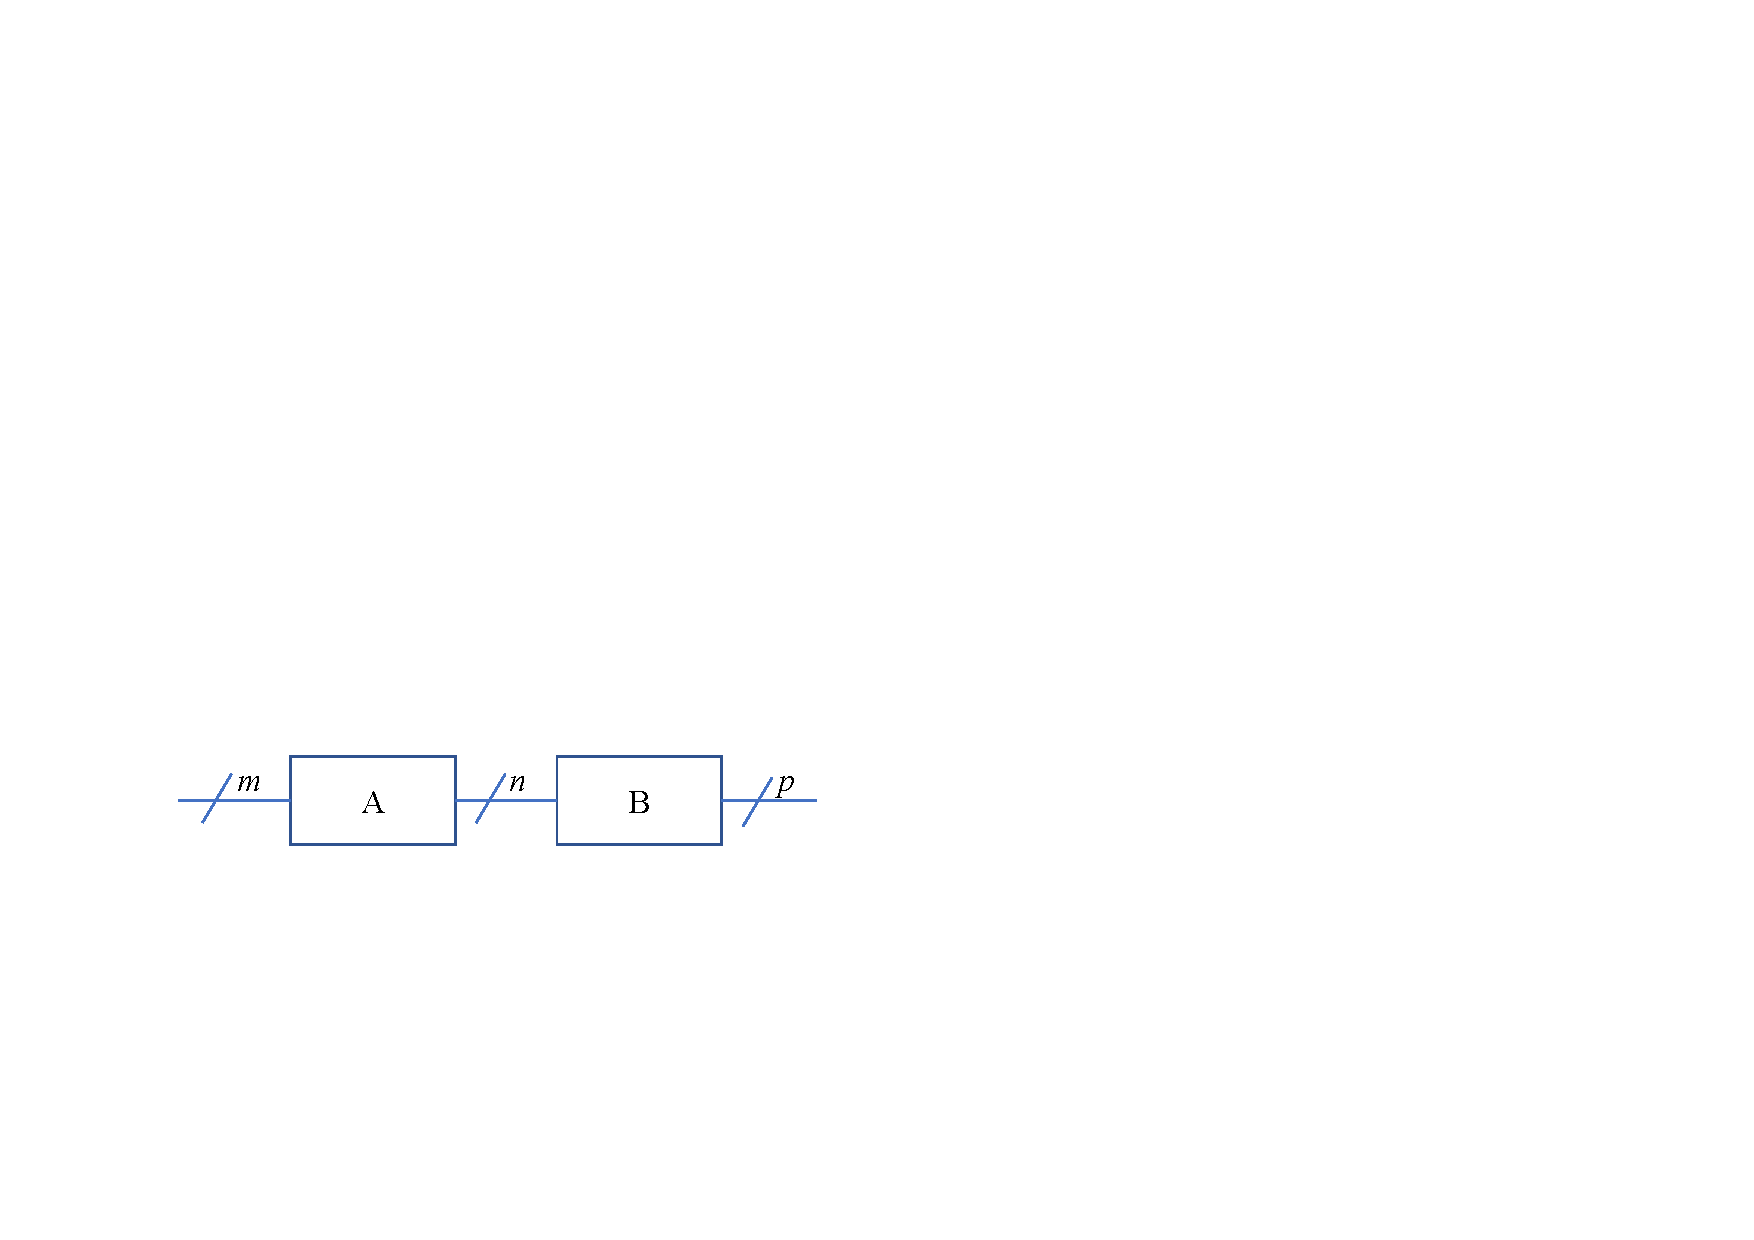
\includegraphics[width=0.3\textwidth]{sequential}
		\label{subfig:sequential}}
	\hspace{0.05\textwidth}
	\subfloat[Parallel operation]
	{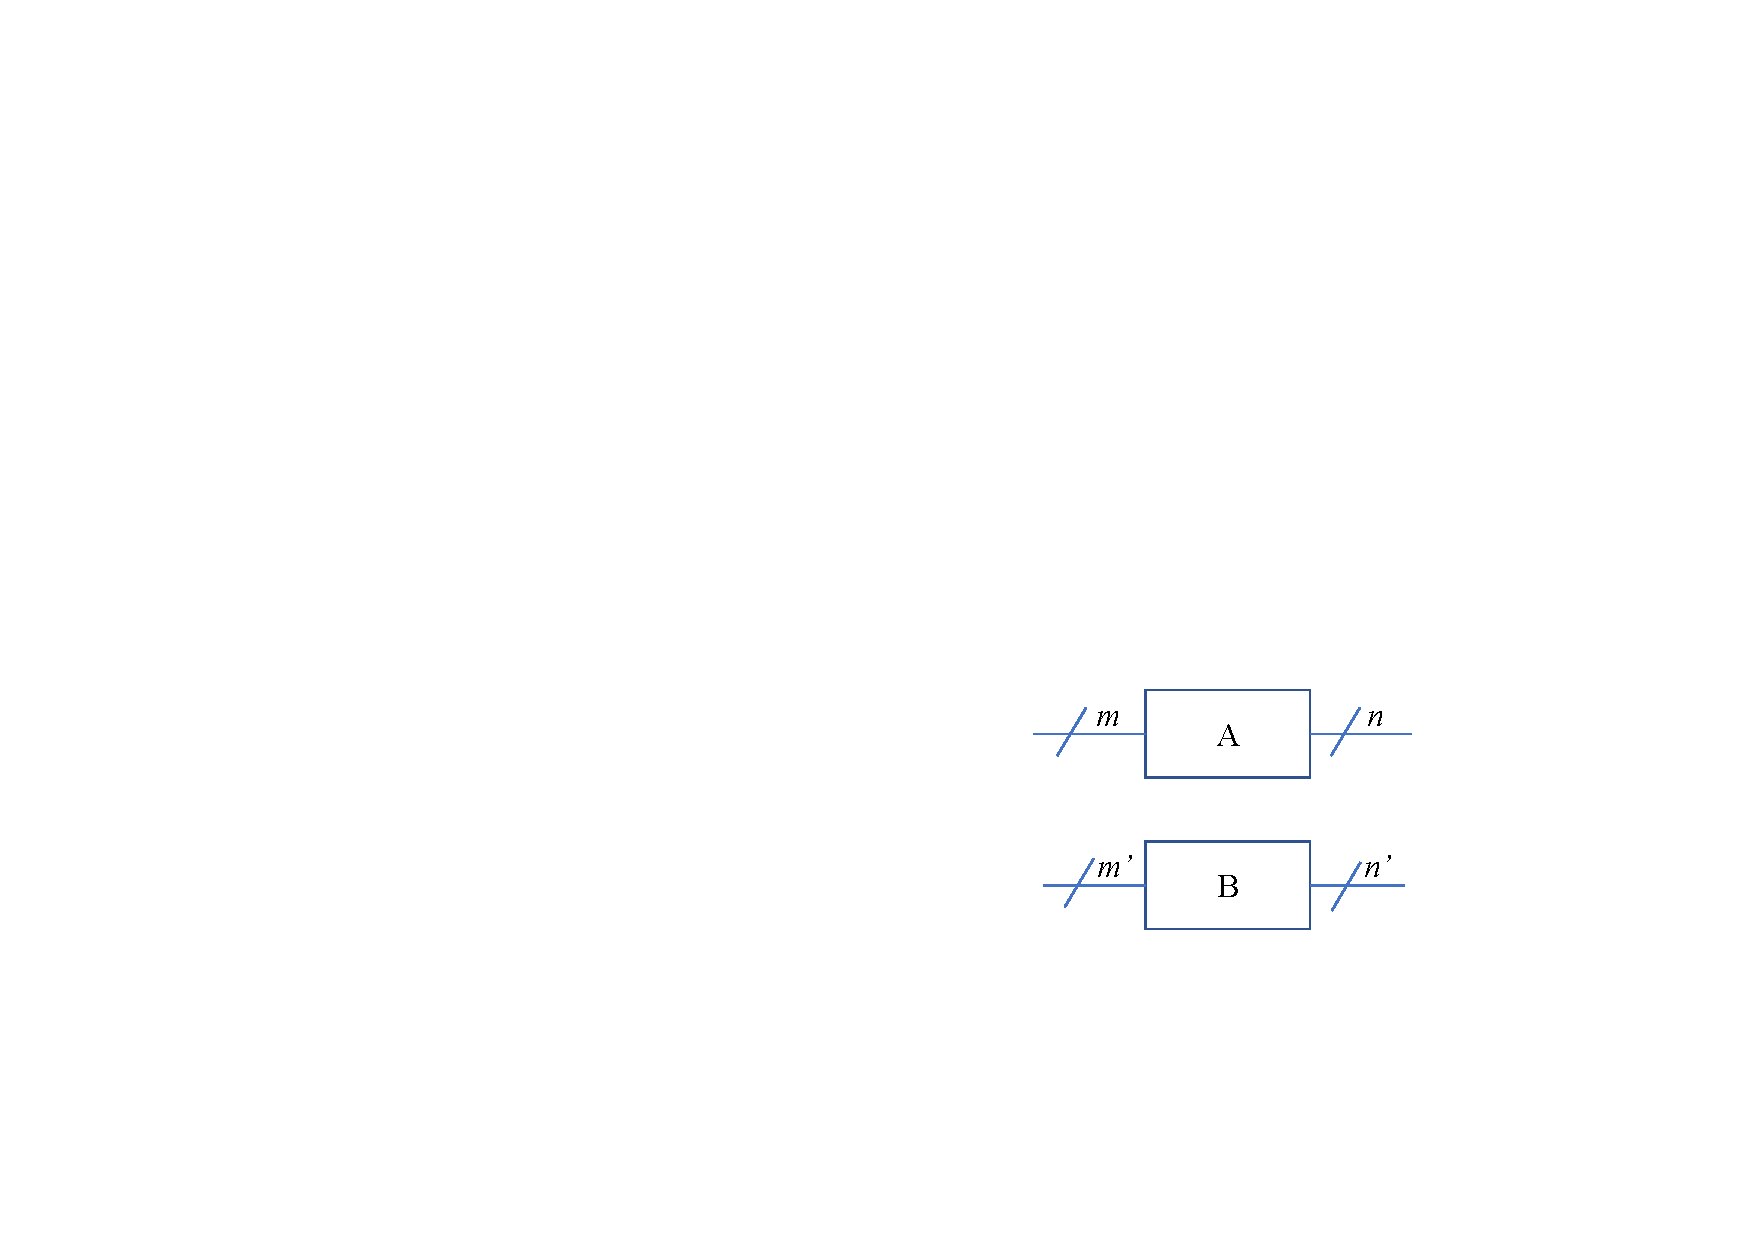
\includegraphics[width=0.2\textwidth]{parallel}
		\label{subfig:parallel}}
	\hspace{0.05\textwidth}
	\subfloat[Mixed operation]
	{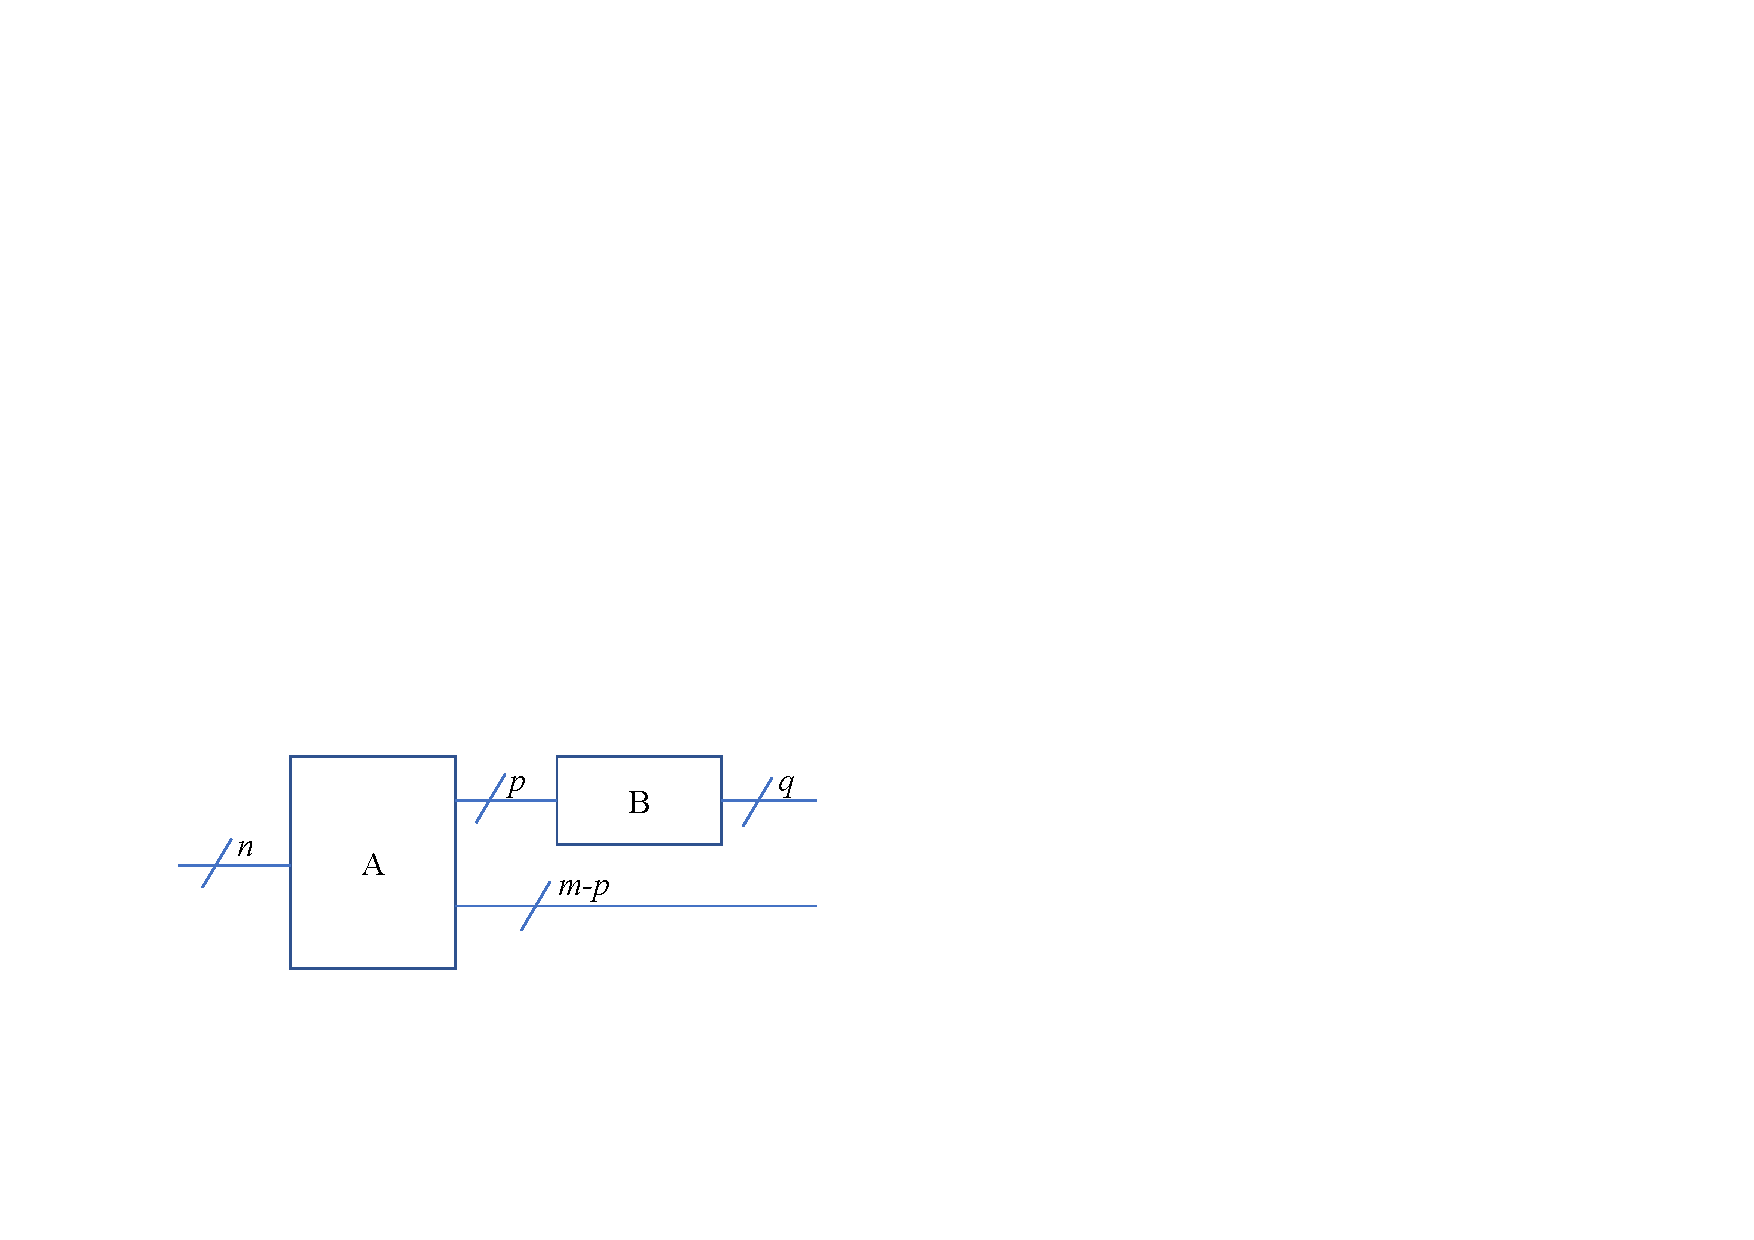
\includegraphics[width=0.35\textwidth]{mixed}
		\label{subfig:mixed}}
	\caption{Sequential, parallel and mixed operations.}
	\label{fig:sequential-parallel-mixed-operations}
\end{figure}

\textbf{Parallel operation.} Besides sequential operations, there are parallel operations as shown in Figure \ref{subfig:parallel}. Here we have A acting on some bits and B on others. This will be represented by $\textrm{A}\otimes \textrm{B}$. Let us be exact with the number of inputs and the number of outputs. A will be of size $2^n\times2^m$. B will be of size $2^{n'}\times2^{m'}$, $\textrm{A}\otimes \textrm{B}$ is of size $2^n2^{n'} = 2^{n+n'}\times 2^m2^{m'} = 2^{m+m'}$ .

\textbf{Mixed operation.} Take Figure \ref{subfig:mixed} as an example, let A be an operation that takes $n$ inputs and gives $m$ outputs. Let B take $p < m$ of these outputs and leave the other $m-p$ outputs alone. B outputs $q$ bits. A is a $2^m\times 2^n$ matrix. B is a $2^q\times 2^p$ matrix. As nothing should be done to the $m-p$ bits, we might represent this as the $2^{m-p}\times 2^{m-p}$ identity matrix $\textrm{I}_{m-p}$. We do not draw any gate for the identity matrix. The entire circuit can be represented by the following matrix:
\begin{equation}
	(\textrm{B}\otimes \textrm{I}_{m-p})\times \textrm{A}
\end{equation}

\begin{example}[Example 1 for mixed operation]{ex:mixed-ex1}
	Consider the circuit:
	\begin{minipage}{0.8\textwidth}
		\hspace{1cm}
		\begin{circuitikz}
			% NOT gate
			\draw (2,2) node[not port] (mynot) {};
			\draw (mynot.out) -- ++(0.5,0) coordinate (notout);
			
			% AND gate
			\draw (2.6,0) node[and port] (myand) {};
			\draw (myand.out) -- ++(0.5,0) coordinate (andout);
			
			% OR gate
			\draw (6,1) node[or port] (myor) {};
			\draw (myor.in 1) -- ++(-0.5,0) node[left] {$$};
			\draw (myor.in 2) -- ++(-0.5,0) node[left] {$$};
			\draw (notout) |- (myor.in 1);
			\draw (andout) |- (myor.in 2);
			\draw (myor.out) -- ++(0.5,0) node[right] {$$};
		\end{circuitikz}
		\vspace{0.5cm}
	\end{minipage}
	
	This is represented by 
	\begin{equation}
		\textrm{OR}\times(\textrm{NOT}\times \textrm{AND})
	\end{equation}
	Let us see how the operations look like as matrices. We first calculate the parallel part:
	\begin{equation}
		\textrm{NOT}\otimes\textrm{AND}=
		\begin{bmatrix}
			0 & 1\\
			1 & 0
		\end{bmatrix}\otimes
		\begin{bmatrix}
			1 & 1 & 1 & 0\\
			0 & 0 & 0 & 1
		\end{bmatrix}=
		\begin{bmatrix}
			0 & 0 & 0 & 0 & 1 & 1 & 1 & 0\\
			0 & 0 & 0 & 0 & 0 & 0 & 0 & 1\\
			1 & 1 & 1 & 0 & 0 & 0 & 0 & 0\\
			0 & 0 & 0 & 1 & 0 & 0 & 0 & 0
		\end{bmatrix}
	\end{equation} 	
	And then we calculate the whole circuit:
	\begin{equation}
		\textrm{OR}\times(\textrm{NOT}\otimes \textrm{AND})=
		\begin{bmatrix}
			0 & 0 & 0 & 0 & 1 & 1 & 1 & 0\\
			1 & 1 & 1 & 1 & 0 & 0 & 0 & 1
		\end{bmatrix}
	\end{equation} 	
\end{example}

\begin{example}[Example 2 for mixed operation]{ex:mixed-ex2}
	Consider the circuit:
	\begin{minipage}{0.8\textwidth}
		\hspace{1cm}
		\begin{circuitikz}
			% First NOT gate
			\draw (0,0) node[not port] (not1) {};
			\draw (not1.out) -- ++(0.5,0) coordinate (not1out);
			
			% Second NOT gate
			\draw (0,-2) node[not port] (not2) {};
			\draw (not2.out) -- ++(0.5,0) coordinate (not2out);
			
			% AND gate
			\draw (4,-1) node[and port] (and) {};
			\draw (and.out) -- ++(0.5,0) coordinate (andout);
			
			% NOT gate (last part)
			\draw (6,-1) node[not port] (not3) {};
			\draw (not3.in) -- ++(-0.5,0) coordinate (not3in);
			\draw (andout) -- (not3in);
			
			% Connections
			\draw (not1out) |- (and.in 1);
			\draw (not2out) |- (and.in 2);
		\end{circuitikz}
		\vspace{0.5cm}
	\end{minipage}
	This is represented by 
	\begin{equation}
		\textrm{NOT}\times\textrm{AND}\times(\textrm{NOT}\otimes \textrm{NOT})
	\end{equation}
	Let us see how the operations look like as matrices. We first calculate the parallel part:
	\begin{equation}
		\textrm{NOT}\otimes\textrm{NOT}=
		\begin{bmatrix}
			0 & 1\\
			1 & 0
		\end{bmatrix}\otimes
		\begin{bmatrix}
			0 & 1\\
			1 & 0
		\end{bmatrix}=
		\begin{bmatrix}
			0 & 0 & 0 & 1\\
			0 & 0 & 1 & 0\\
			0 & 1 & 0 & 0\\
			1 & 0 & 0 & 0
		\end{bmatrix}
	\end{equation} 	
	And then we calculate the whole circuit $\textrm{NOT}\times\textrm{AND}\times(\textrm{NOT}\otimes \textrm{NOT})$:
	\begin{equation}
		\begin{bmatrix}
			0 & 1\\
			1 & 0
		\end{bmatrix}\times
		\begin{bmatrix}
			1 & 1 & 1 & 0\\
			0 & 0 & 0 & 1
		\end{bmatrix}\times
		\begin{bmatrix}
			0 & 0 & 0 & 1\\
			0 & 0 & 1 & 0\\
			0 & 1 & 0 & 0\\
			1 & 0 & 0 & 0
		\end{bmatrix}=
		\begin{bmatrix}
			1 & 0 & 0 & 0\\
			0 & 1 & 1 & 1
		\end{bmatrix}
	\end{equation} 	
\end{example}
%general gate

\section{Reversible Gates}
In the quantum world, all operations that are not measurements are reversible and are represented by unitary matrices. The AND operation is not reversible. Given an output of $\ket{0}$ from AND, one cannot determine if the input was $\ket{00}$, $\ket{01}$, or $\ket{10}$. So from an output of the AND gate, one cannot determine the
input and hence AND is not reversible. In contrast, the NOT gate and the identity
gates are reversible. 

Reversible gates have a history that predates quantum computing. In the 1960s, Rolf Landauer analyzed computational processes and showed that erasing information, as opposed to writing information, is what causes energy loss and heat. This notion has come to be known as the \textbf{Landauer’s principle}.

We have found that erasing information is an irreversible, energy-dissipating
operation. In the 1970s, Charles H. Bennett continued along these lines of thought.
If erasing information is the only operation that uses energy, then a computer that
is reversible and does not erase would not use any energy. Bennett started working
on reversible circuits and programs.

A reversible circuit has exactly as many outputs as inputs. Each input can be reconstructed from the output; no bits are lost, so reversible circuits will not give off heat from bit loss.

\subsection{CNOT gate}
What examples of reversible gates are there? We have already seen that the identity gate and NOT gates are reversible. What else is there? Consider the following controlled-NOT gate shown in Figure \ref{fig:cnot} (a):

\begin{figure}[h]
	\centering
	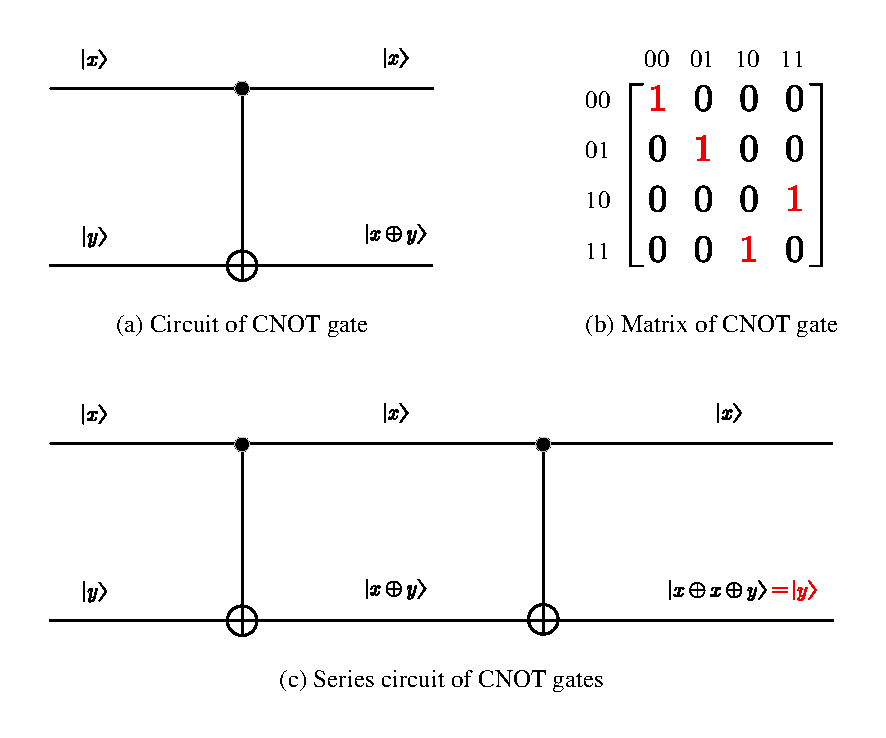
\includegraphics[width=0.8\textwidth]{cnot}
	\caption{The circuit (a), matrix (b), and reversion (c) of CNOT gate.}
	\label{fig:cnot}
\end{figure}

This gate has two inputs and two outputs. The top input is the control bit. It controls what the output will be. If $\ket{x}=\ket{0}$, then the bottom output of $\ket{y}$ will be the same as the input. If $\ket{x}=\ket{1}$, then the bottom output will be the opposite. If we write the top qubit first and then the bottom qubit, then the controlled-NOT gate takes $\ket{x,y}$ to $\ket{x,x\oplus y}$, where $\oplus$ is the binary ``exclusive or'' operation. The matrix that corresponds to this reversible gate is shown in Figure \ref{fig:cnot} (b).

CNOT gate can be reversed by itself as shown in Figure \ref{fig:cnot} (c). State $\ket{x,y}$ goes to $\ket{x,x\oplus y}$, which further goes to $\ket{x,x\oplus(x\oplus y)}$. This last
state is equal to $\ket{x,(x\oplus x)\oplus y}$ because $\oplus$ is associative. Because $x\oplus x$ is always equal to $0$, this state reduces to the original $\ket{x,y}$.


\subsection{Toffoli gate}
Toffoli gate extends CNOT gate's function by using two controlling bits. The bottom bit flips only when \textit{both} of the top two bits are in state $\ket{1}$. We can write this operation as taking state $\ket{x,y,z}$ to $\ket{x,y,z\oplus (x\wedge y)}$. The circuit and matrix representations of Toffoli gate is shown in Figure \ref{fig:toffoli} (a) and (b). 

\begin{figure}[h]
	\centering
	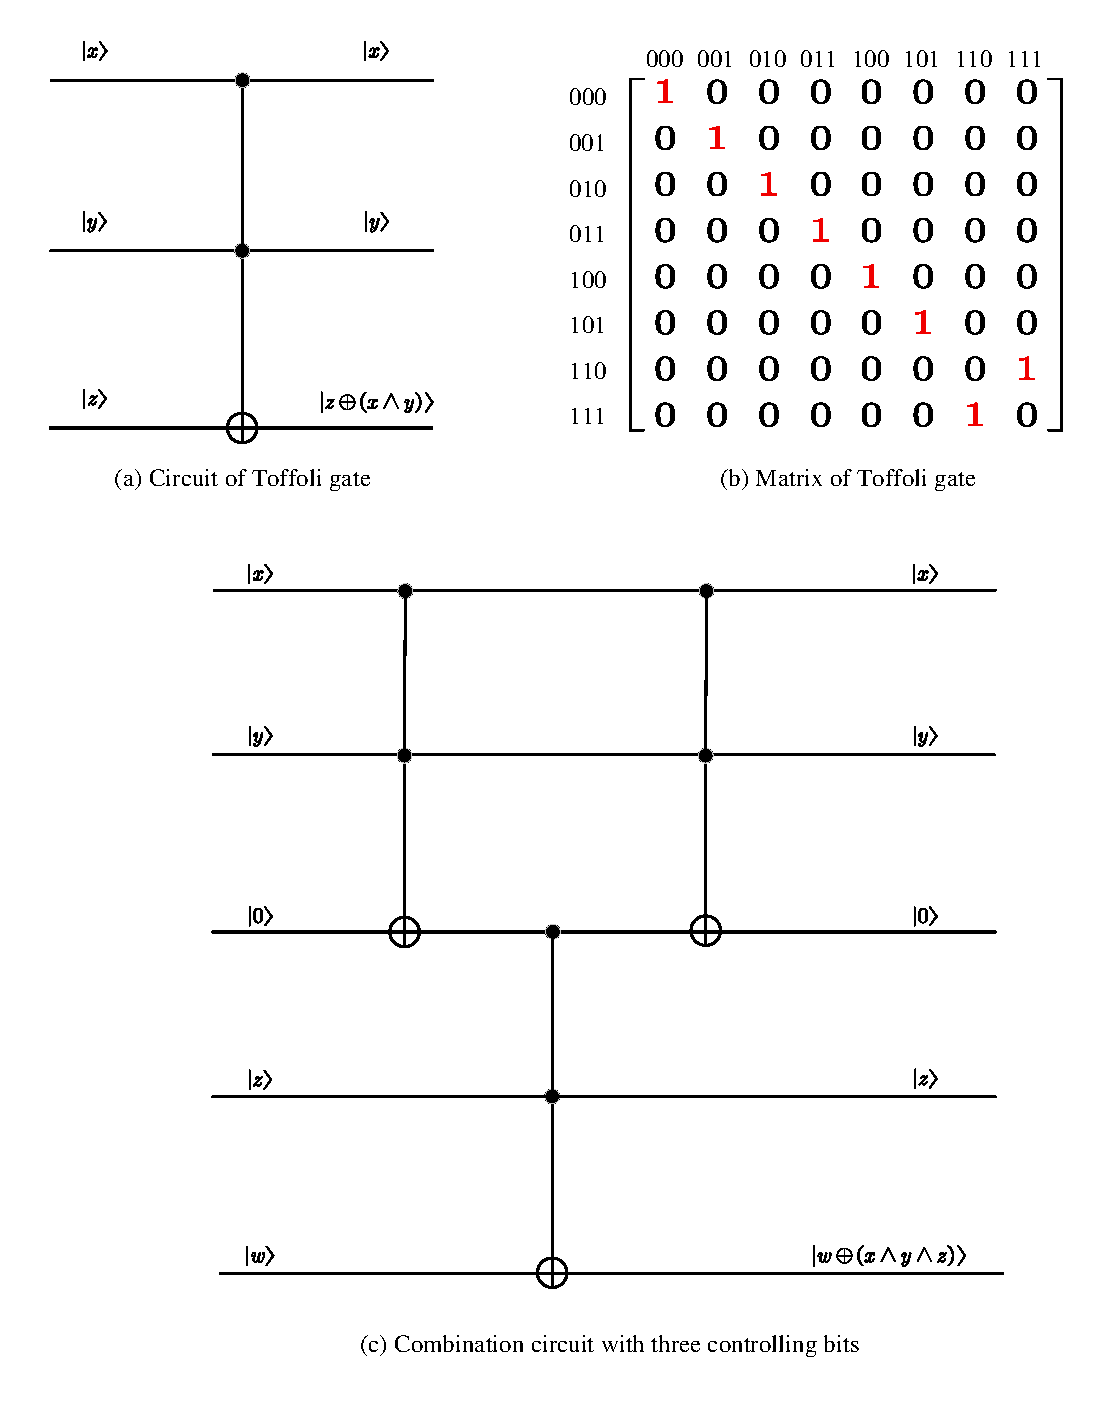
\includegraphics[width=0.75\textwidth]{toffoli}
	\caption{The circuit (a), matrix (b), and combination circuit (c) of Toffoli gate.}
	\label{fig:toffoli}
\end{figure}

The NOT gate has no controlling bit, the CNOT gate has one controlling bit, and the Toffoli gate has two controlling bits. We can go on with this by with the combination circuit shown in Figure \ref{fig:toffoli} (c). 

\begin{figure}[h]
	\centering
	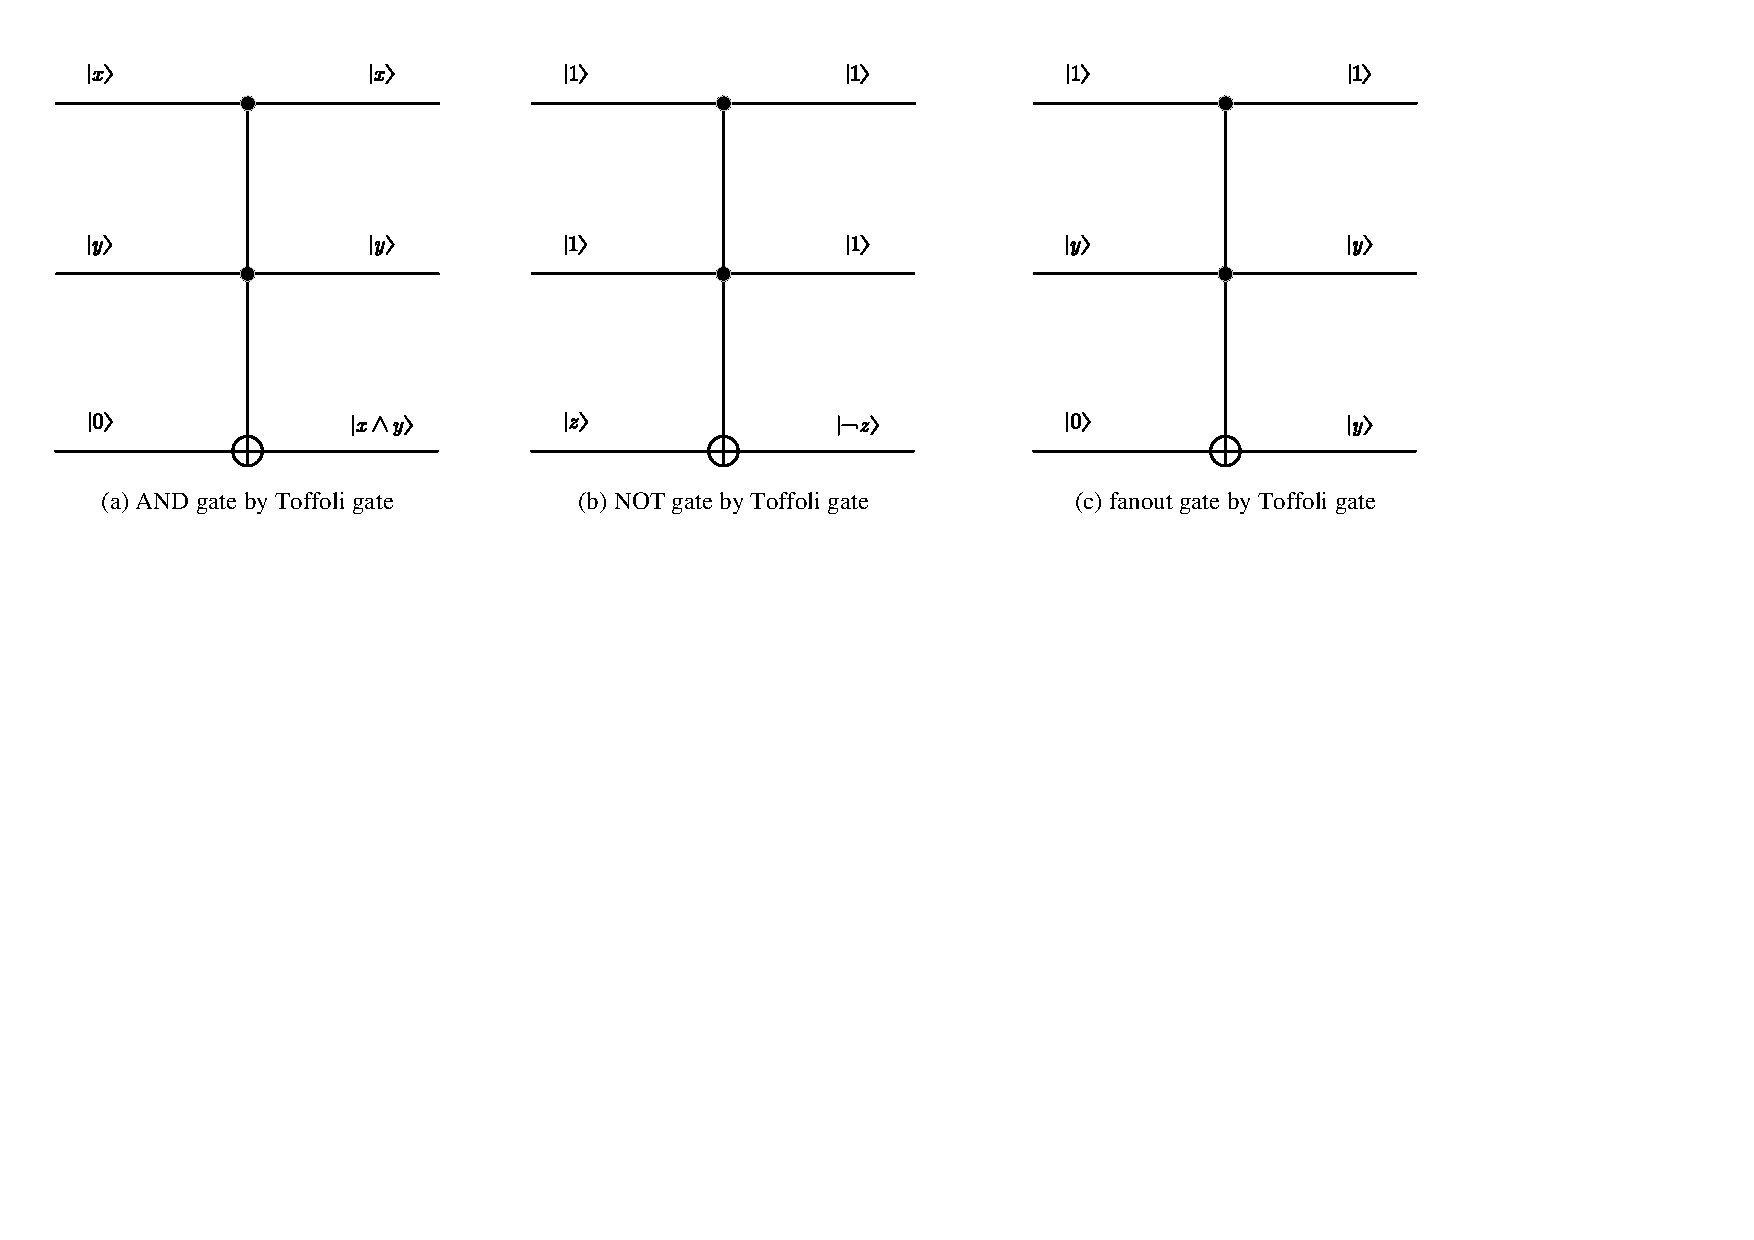
\includegraphics[width=0.9\textwidth]{toffoli-universal}
	\caption{AND gate (a), NOT gate (b), and fanout gate (c) by Toffoli gate.}
	\label{fig:toffoli-universal}
\end{figure}

One reason why the Toffoli gate is interesting is that it is universal. In other words, with copies of the Toffoli gate, we can make any logical gate. In order to see that the Toffoli gate is universal, we will show that it can be used to make both the AND and NOT gates as shown in Figure \ref{fig:toffoli-universal} (a) and (b). Specifically, the AND gate is obtained by setting the bottom $\ket{z}$ input to $\ket{0}$, and the bottom output will then be $\ket{x\wedge y}$. The NOT gate is obtained by setting the top two inputs to $\ket{1}$, and bottom output will be $\ket{(1\wedge 1)\oplus z}=\ket{1\oplus z}=\ket{\neg z}$. 

Moreover, in order to construct all gates, we must also have a way of producing a fanout of values. In other words, a gate is needed that inputs a value and outputs two of the same values. This can be obtained by setting $\ket{x}$ to $\ket{1}$ and $\ket{z}$ to $\ket{0}$. This makes the output $\ket{1,y,y}$. 


\subsection{Fredkin gate}
Another interesting reversible gate is the Fredkin gate. The Fredkin gate also has three inputs and three outputs as shown in Figure \ref{fig:fredkin} (a). The top $\ket{x}$ input is the control input. The output is always the same $\ket{x}$. If $\ket{x}$
is set to $\ket{0}$, then $\ket{y'}=\ket{y}$ and $\ket{z'}=\ket{z}$, \textit{i.e.}, the values stay the same. If, on the other hand, the control $\ket{x}$ is set to $\ket{1}$, then the outputs are reversed: $\ket{y'}=\ket{z}$ and $\ket{z'}=\ket{y}$. In short, $\ket{0, y, z} \mapsto \ket{0,y,z}$ and $\ket{1, y, z} \mapsto \ket{1,z,y}$.

\begin{figure}[h]
	\centering
	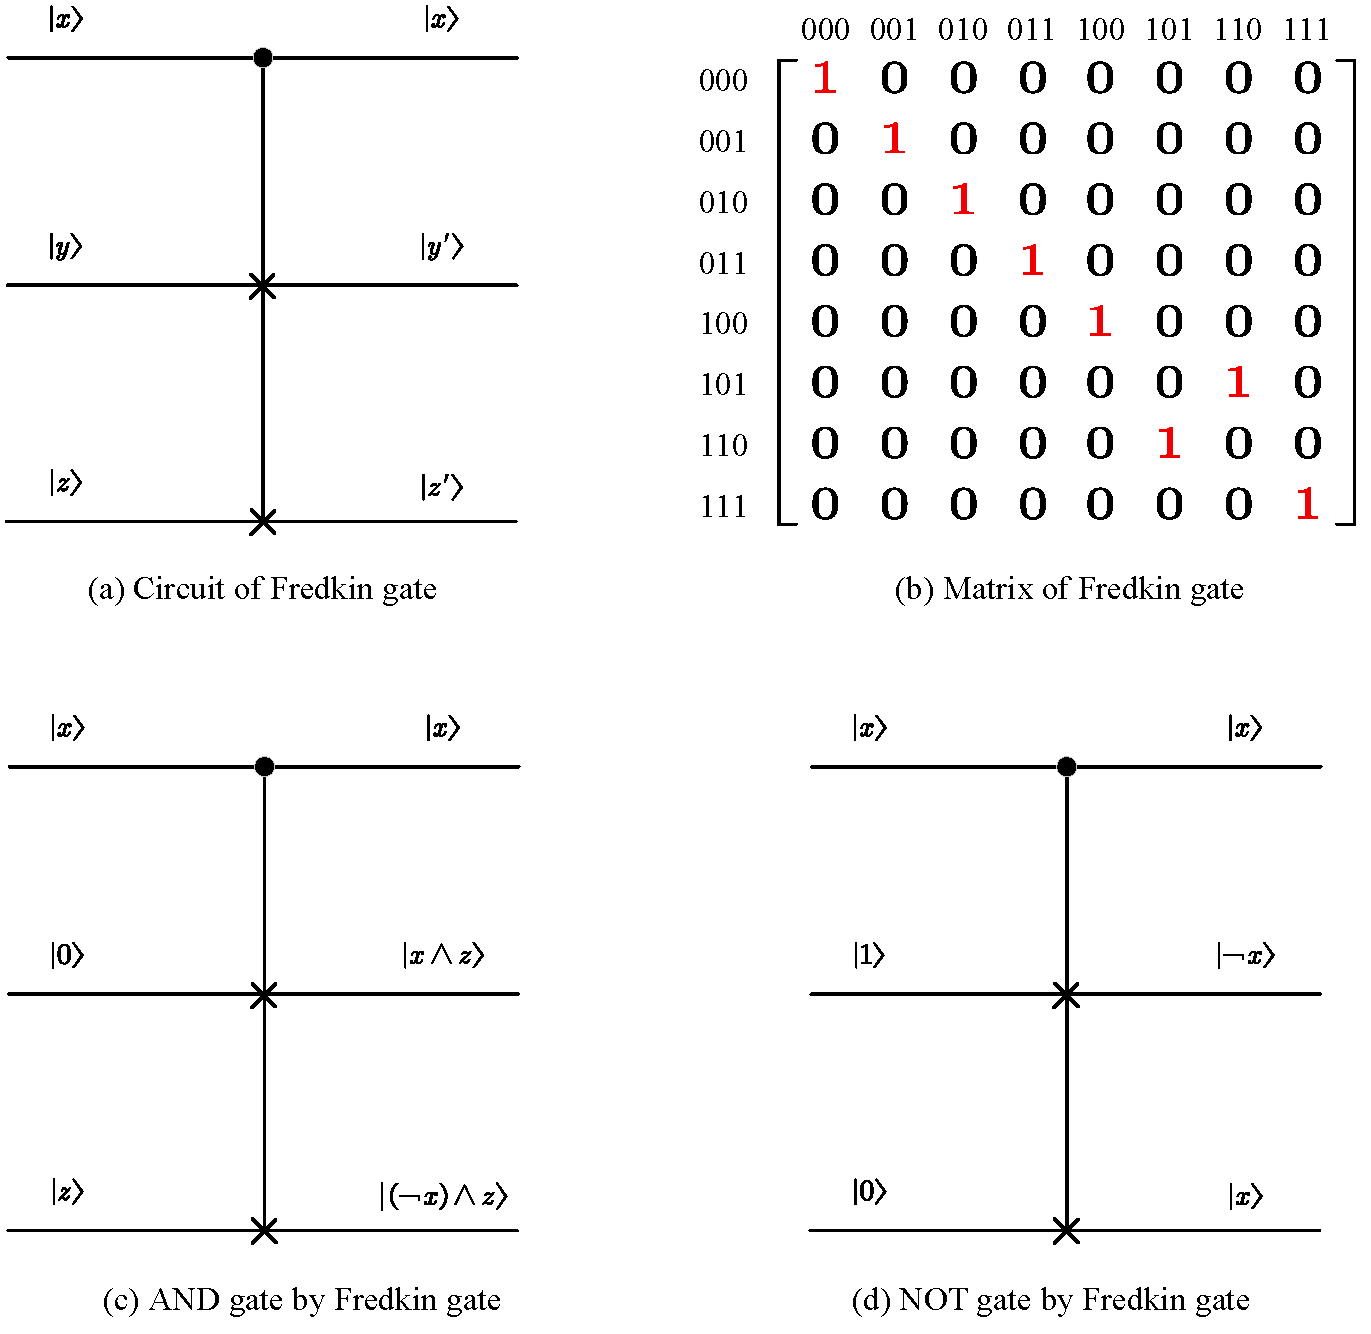
\includegraphics[width=0.9\textwidth]{fredkin}
	\caption{The circuit (a), matrix (b) of Fredkin gate and its functional equivalence to AND gate (c), and NOT and fanout gate (d).}
	\label{fig:fredkin}
\end{figure}

The matrix that corresponds to the Fredkin gate is shown in Figure \ref{fig:fredkin} (b), from which we can see that the Fredkin gate is its own inverse. The Fredkin gate is also universal. By setting $\ket{y}$ to $\ket{0}$ as shown in Figure \ref{fig:fredkin} (c). The NOT gate and the fanout gate can be obtained by setting $\ket{y}$ to $\ket{1}$ and $\ket{z}$ to $\ket{0}$ as shown in Figure \ref{fig:fredkin} (d). 

So both the Toffoli and the Fredkin gates are universal. Not only are both reversible gates; a glance at their matrices indicates that they are also unitary. 


\section{Quantum Gates}
\textbf{quantum gate} is simply an operator that acts on qubits. Such
operators will be represented by unitary matrices.

We have already worked with some quantum gates such as the identity operator I, the Hadamard gate H, the NOT gate, the CNOT gate, the Toffoli gate, and the Fredkin gate. What else is there? Here we discuss some important quantum gates:

\begin{itemize}
	\item \textbf{Pauli matrices}. They occur everywhere in quantum mechanics and quantum computing. Note that the X matrix is nothing more than our NOT matrix.
	\begin{equation}
		\mathrm{X}=\begin{bmatrix}
			0 & 1\\
			1 & 0
		\end{bmatrix},\quad
		\mathrm{Y}=\begin{bmatrix}
			0 & -i\\
			i & 0
		\end{bmatrix},\quad
		\mathrm{Z}=\begin{bmatrix}
			1 & 0\\
			0 & -1
		\end{bmatrix}
	\end{equation}

	\item \textbf{Square root of NOT}. It is a one-qubit quantum gate and is denoted as $\sqrt{\mathrm{NOT}}$. The matrix representation of this gate is
	\begin{equation}
		\sqrt\mathrm{NOT}=\frac{1}{\sqrt{2}}\begin{bmatrix}
			1 & -1\\
			1 & 1
		\end{bmatrix}
	\end{equation}

	\item \textbf{Hardmard gates}. It is defined as 
	\begin{equation}
		\mathrm{H}=\begin{bmatrix}
			\frac{1}{\sqrt{2}} & \frac{1}{\sqrt{2}}\\
			\frac{1}{\sqrt{2}} & -\frac{1}{\sqrt{2}}
		\end{bmatrix}
	\end{equation}
	The Hardmard gate has two important properties in quantum algorithm (see Example \ref{ex:H gate}). First, we can transition into superposition from classic state through Hardmard gate. Second, we can transition out of superposition without measurement with the help of Hardmard gate. 

	\item \textbf{Phase shift gate}. It is defined as  
	\begin{equation}
		R(\theta)=\begin{bmatrix}
			1 & 0\\
			0 & e^{i\theta}
		\end{bmatrix}
	\end{equation}
	This gate performs the following operation on an arbitrary qubit:
	\begin{equation}
		\cos(\theta')\ket{0}+e^{i\phi}\sin{\theta'}\ket{1}=
		\begin{bmatrix}
			\cos(\theta')\\
			e^{i\phi}\sin{\theta'}
		\end{bmatrix}\mapsto
		\begin{bmatrix}
			\cos(\theta')\\
			e^{i(\theta+\phi)}\sin{\theta'}
		\end{bmatrix}
	\end{equation}
	This corresponds to a rotation that leaves the latitude alone and just changes the longitude. The new state of the qubit will remain unchanged. Only the phase will change.
	
	\item \textbf{Controlled-U gate}. It is equivalent to an IF–THEN statement. If a certain (qu)bit is true, then a particular operation should be performed, otherwise the operation is not
	performed. For every $n$-qubit unitary operation U, we can create a unitary $(n+1)$-qubit operation \textbf{controlled}-U or $^CU$:
	\begin{equation}
		^CU=
		\begin{bmatrix}
			1 & 0 & 0 & 0\\
			0 & 1 & 0 & 0\\
			0 & 0 & a & b\\
			0 & 0 & c & d\\
		\end{bmatrix}
	\end{equation}

	\item \textbf{Deutsch gate}. It is very similar to the Toffoli gate. If the inputs $\ket{x}$ and $\ket{y}$ are both $\ket{1}$, then the phase shift operation $R(\theta)$ will act on the $\ket{z}$ input. Otherwise, the $\ket{z}$ will simply be the same as the $\ket{z}$. When $\theta$ is not a rational multiple of $\pi$, $D(\theta)$ by itself is a universal three-qubit quantum gate. In other words, $D(\theta)$ will be able to mimic every other
	quantum gate.
\end{itemize}

Up to now, we have discussed classic gates, reversible gates and quantum gates. Their relationship can be illustrated by the following Figure \ref{fig:gate-relation}.

\begin{figure}[h]
	\centering
	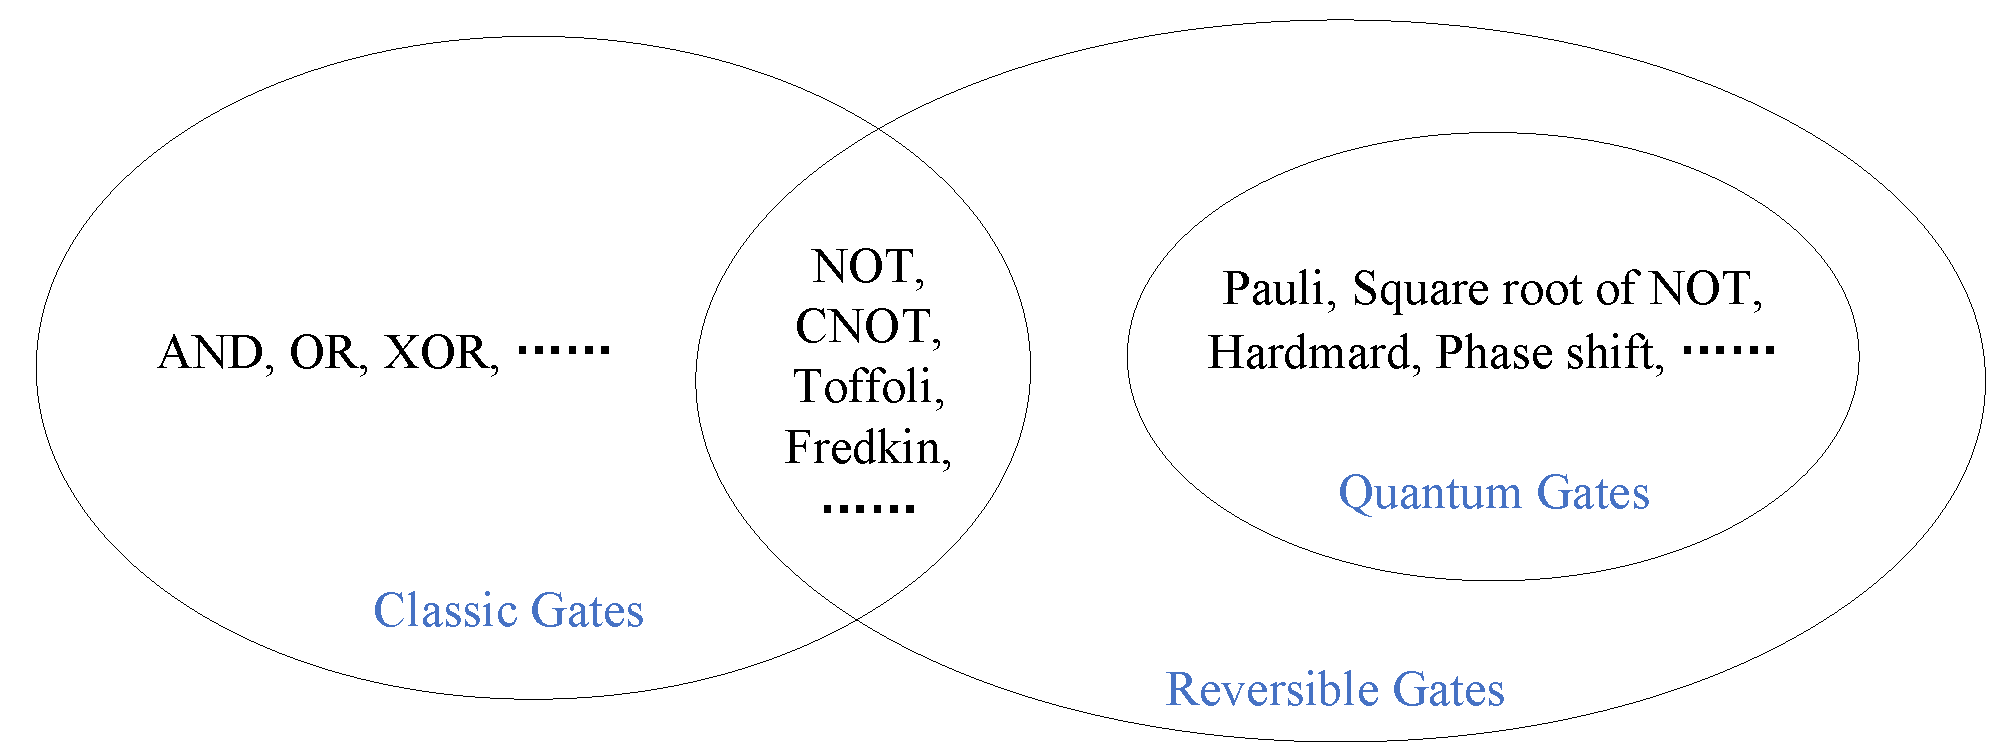
\includegraphics[width=0.9\textwidth]{gate-relation}
	\caption{The relation of various gates.}
	\label{fig:gate-relation}
\end{figure}

\section{Bloch Ball}
\section{The Bell Circuit}
\subsection{Superdense coding}
\subsection{Quantum teleportation}



\curinstructor{Chao Liang}

\ifx\flag\undefined
	\end{document}
\else